% ============================================================================
% SECTION 2: FRAMEWORK
% ============================================================================

\section{Framework}
\label{sec:method}

\subsection{Problem Definition}
\label{sec:problem}

Given a query $q$ and a model pool $\mathcal{M}=\{1,\ldots,M\}$, the router selects a model $m\in\mathcal{M}$ to maximize a utility that trades off predicted quality, cost, and latency:
\begin{equation}
\pi(q) = \argmax_{m \in \mathcal{M}} \left[ \hat{Q}(q, m) - \lambdacost \cdot C_m - \lambdalat \cdot L_m \right]
\label{eq:utility}
\end{equation}
where $\hat{Q}(q, m) \in [0,1]$ is the predicted quality (accuracy), $C_m$ is cost in dollars per 1k tokens, $L_m$ is latency in milliseconds, and $\lambdacost,\lambdalat$ are sensitivity parameters that scale dollar costs and millisecond latencies into comparable utility units. The challenge is that $\hat{Q}$ is initially unknown and must be learned online, but naive cold-start exploration can waste substantial budget before converging.

\subsection{System Architecture}
\label{sec:architecture}

Our system has two asynchronous paths: (1) a \textbf{Hot Path} that performs millisecond-scale routing; and (2) a \textbf{Cold Path} that performs delayed quality assessment and updates the router.

\paragraph{Context Embedding.} Each query is mapped to an embedding $\mathbf{x}=\phi(q)\in\mathbb{R}^{384}$ using a sentence transformer (all-MiniLM-L6-v2), encoding the prompt's semantic representation in the embedding space.

\paragraph{Disjoint LinUCB.} Each model $m$ maintains: $\mathbf{A}_m \in \mathbb{R}^{d \times d}$ (covariance) and $\mathbf{b}_m \in \mathbb{R}^{d}$ (reward accumulator). Predicted quality with exploration bonus:
\begin{equation}
\hat{Q}(q, m) = \underbrace{\boldsymbol{\theta}_m^\top \mathbf{x}}_{\text{exploitation}} + \underbrace{\alpha \sqrt{\mathbf{x}^\top \mathbf{A}_m^{-1} \mathbf{x}}}_{\text{exploration}}
\label{eq:ucb}
\end{equation}
where $\boldsymbol{\theta}_m = \mathbf{A}_m^{-1} \mathbf{b}_m$ encodes model $m$'s learned strengths through pure online learning. Figure~\ref{fig:architecture} illustrates the complete system architecture, showing how user queries flow through feature extraction and route through an 81-model pool with continuous online feedback, converging to optimal routing within $\sim$200 interactions.

\begin{figure}[t]
    \centering
    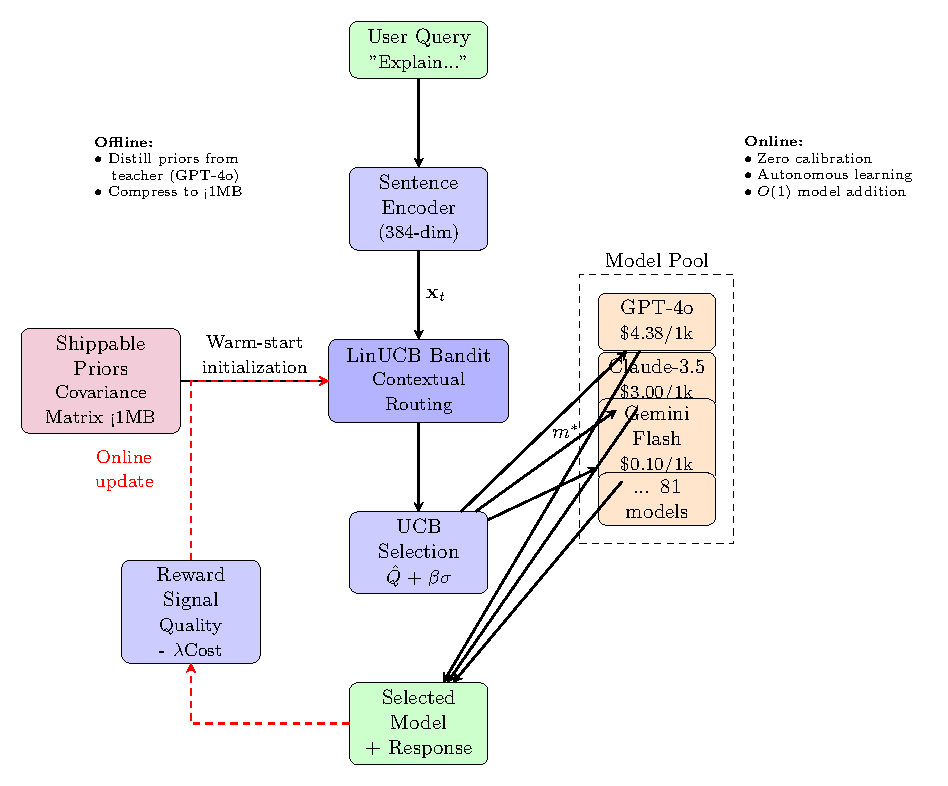
\includegraphics[width=\columnwidth]{figures/architecture_diagram.pdf}
    \caption{\textbf{BanditGPT System Architecture.} The system accepts user queries, extracts contextual features via sentence encoder, initializes with metadata-guided cold start for zero-benchmark deployment, selects from an 81-model pool via UCB, and updates online via reward feedback. Metadata initialization (cost, context, benchmarks) provides constraint enforcement and light quality heuristics from Day 0, while online learning adapts quality preferences to deployment-specific patterns. Model addition requires only public metadata, enabling $O(1)$ registration without offline profiling.}
    \label{fig:architecture}
\end{figure}

\paragraph{Real-Time Learning.} On feedback $(m, \mathbf{x}, r)$, rank-one updates in $O(d^2)$:
\begin{align}
\mathbf{A}_m &\leftarrow \mathbf{A}_m + \mathbf{x}\mathbf{x}^\top, \quad
\mathbf{b}_m \leftarrow \mathbf{b}_m + r \cdot \mathbf{x}
\label{eq:update}
\end{align}

\subsection{Algorithm Mechanics: Disjoint LinUCB}
\label{sec:linucb}

To solve the routing problem efficiently under uncertainty, we employ the Disjoint Linear Upper Confidence Bound (LinUCB) algorithm. We choose the \emph{disjoint} variant because LLM capabilities are often uncorrelated across disjoint architectures (e.g., a ``Math'' specialist like Grok has a completely different feature-response surface than a ``Creative'' model like Claude). Sharing parameters across arms (Hybrid LinUCB) would incorrectly bias the router to assume correlated performance where none exists.

For each model (arm) $k$, we maintain a learned weight vector $\hat{\boldsymbol{\theta}}_k$ computed from ridge regression of historical contexts $\mathbf{x}$ onto rewards $r$:
\begin{equation}
\hat{\boldsymbol{\theta}}_k = \mathbf{A}_k^{-1} \mathbf{b}_k
\end{equation}
where $\mathbf{A}_k$ is the covariance matrix (initialized as $\mathbf{I}_d$) and $\mathbf{b}_k$ is the reward vector. The algorithm selects the model that maximizes the Upper Confidence Bound (UCB) of the estimated reward:
\begin{equation}
k_t = \argmax_{k \in \mathcal{K}} \left( \mathbf{x}_t^\top \hat{\boldsymbol{\theta}}_k + \alpha \sqrt{\mathbf{x}_t^\top \mathbf{A}_k^{-1} \mathbf{x}_t} \right)
\end{equation}
The first term ($\mathbf{x}_t^\top \hat{\boldsymbol{\theta}}_k$) represents \textbf{Exploitation} (predicted quality), while the second term represents \textbf{Exploration} (uncertainty). The hyperparameter $\alpha$ controls the aggressiveness of exploration.

\subsection{Regret Formulation}
\label{sec:regret}

We evaluate learning efficiency through \textbf{cumulative regret}, defined as the total reward differential between the oracle optimal policy and the learned policy over $T$ rounds:
\begin{equation}
R_T = \sum_{t=1}^T \left( r(\mathbf{x}_t, k^*) - r(\mathbf{x}_t, k_t) \right)
\end{equation}
where $k^*$ denotes the optimal model for query $\mathbf{x}_t$ (determined via oracle ground truth), $k_t$ represents the model selected by \ours{}, and $r(\cdot)$ is the realized reward. This metric quantifies the opportunity cost of exploration---the performance degradation incurred while the system gathers information about suboptimal models. Minimizing $R_T$ indicates rapid convergence to optimal model selection across diverse prompt types. Our cold-start initialization with $\mathbf{A}_k = \lambda \mathbf{I}$ and $\mathbf{b}_k = \mathbf{0}$ ensures high uncertainty, forcing balanced exploration and avoiding the negative transfer observed with offline-calibrated covariance matrices (\S\ref{sec:rq1}).

\subsection{User Control: The Tunable Objective ($\lambda$)}
\label{sec:lambda}

Conventional bandit algorithms optimize exclusively for prediction accuracy. However, production environments require explicit control over operational constraints such as budget allocation and service-level agreements. We augment the reward function $r(\mathbf{x}, k)$ to incorporate model cost and latency through user-defined sensitivity parameters:
\begin{equation}
r(\mathbf{x}, k) = \text{Quality}(\mathbf{x}, k) - \lambdacost \cdot \text{Cost}_k - \lambdalat \cdot \text{Latency}_k
\end{equation}
where $\lambdacost$ and $\lambdalat$ are sensitivity parameters that convert operational costs (dollars, milliseconds) into utility penalties commensurate with quality loss. These parameters enable precise control over the cost-quality-latency trade-off space:
\begin{itemize}[leftmargin=*,nosep]
    \item $\lambdacost \to 0$: The system operates in maximum performance mode, selecting frontier models (e.g., GPT-4o) without cost constraints.
    \item $\lambdacost \gg 0$: The effective reward for expensive models decreases substantially. The bandit is incentivized to explore cost-efficient alternatives (e.g., Gemini~Flash~Lite), selecting expensive models only when the predicted quality differential ($\Delta\text{Quality}$) justifies the additional cost penalty ($\lambdacost \cdot \Delta\text{Cost}$).
\end{itemize}
This formulation ensures that cost optimization emerges as an \emph{intrinsic property} of the learned routing policy rather than through heuristic post-processing.

\subsection{Why Contextual Bandits?}
\label{sec:pivot}

Static classification approaches~\cite{ong2024routellm} require retraining when model capabilities evolve. We adopt contextual bandits for three fundamental advantages: (1)~\textbf{Distribution Drift Resilience}---model capabilities shift frequently (e.g., GPT-4o monthly updates); online learning enables continuous adaptation without manual intervention. (2)~\textbf{Domain-Specific Specialization}---the system autonomously discovers local specialists that excel in deployment-specific distributions but remain underrepresented in global benchmarks. (3)~\textbf{Principled Exploration}---LinUCB provably balances exploration and exploitation, achieving near-optimal regret bounds under linear reward assumptions~\cite{abbasi2011improved}.

\subsection{Cold Start by Design}
\label{sec:cold_start}

Unlike offline routing methods that require extensive calibration datasets~\cite{chen2023frugal,ong2024routellm}, our system deploys immediately with zero quality assumptions. Each model initializes with:
\begin{equation}
\mathbf{A}_m = \lambda \mathbf{I}, \quad \mathbf{b}_m = \mathbf{0}
\end{equation}
where $\lambda=1.0$ provides standard ridge regularization and $\mathbf{I}$ is the identity matrix. This high-uncertainty initialization forces balanced exploration across the model pool, allowing the system to discover task-specific rankings through live feedback alone.

\paragraph{Design Rationale.} We intentionally avoid quality priors (benchmarks, pre-training) based on empirical findings (\S\ref{sec:rq1}) showing that offline calibration provides no benefit and often degrades performance through negative transfer effects. Our experiments demonstrate that:
\begin{itemize}[leftmargin=*,nosep]
    \item \textbf{Dense offline training} on 497 prompts causes +32\% regret increase (p=0.08, 5-fold CV)
    \item \textbf{Benchmark initialization} provides no benefit over uniform start (mean -3.6\%, p=0.60)
    \item \textbf{Pure cold start} converges to optimal routing within $\sim$200 interactions
\end{itemize}

\paragraph{Why This Works.} Online learning adapts so rapidly that initialization strategy is irrelevant for long-term performance. Starting cold eliminates: (1)~the risk of negative transfer from mismatched offline data, (2)~the need to collect calibration datasets, and (3)~maintenance overhead when model capabilities evolve. Hard constraints (cost, context limits) are enforced through pre-filtering; quality preferences emerge naturally through online experience.


\subsection{Engineering Viability}
\label{sec:engineering}

\begin{table}[t]
\centering
\small
\caption{\textbf{Latency Breakdown.} Router adds 1.1\% overhead (81 models, 384 dims).}
\label{tab:latency}
\begin{tabular}{lrr}
\toprule
\textbf{Component} & \textbf{P99} & \textbf{\% Total} \\
\midrule
Router Inference & 8.94 ms & 1.1\% \\
Network / API & 50.00 ms & 6.2\% \\
LLM Generation & 750.00 ms & 92.7\% \\
\bottomrule
\end{tabular}
\end{table}

Router overhead is negligible: 8.94ms P99 (Table~\ref{tab:latency}). The $O(d^2)$ matrix operations do not bottleneck; the router adds only 1.1\% to end-to-end latency while enabling substantial cost savings.

\subsection{Zero-Overhead Scalability}
\label{sec:scalability}

A critical limitation of existing routers is their \emph{$O(N)$ scaling cost}: adding a new model requires running calibration benchmarks (FrugalGPT) or re-training a classifier (RouteLLM). In rapidly evolving markets---where new models launch weekly---this creates an operational bottleneck.

\paragraph{Learning Prompt Difficulty Online.} The bandit learns \emph{what makes prompts difficult} directly from live feedback---this knowledge is model-specific and continuously updated. When a new model releases, we simply fetch \textbf{hard constraints} from the OpenRouter API metadata (cost per token, context window, latency percentiles)~\cite{openrouter2024pricing} and register the model. The bandit treats cost and latency as known (eliminating profiling overhead), while autonomously learning the model's quality via online feedback within $\sim$50--100 interactions.

\paragraph{Day-1 Integration Workflow.}
\begin{enumerate}[leftmargin=*,nosep]
    \item \textbf{Release}: Model X launches with claimed Math score 85\%.
    \item \textbf{Registration}: Add to registry with \texttt{min\_quality=85}, cost metadata. Time: seconds.
    \item \textbf{SLA Filter}: Model X is eligible for prompts where quality floor $<85\%$.
    \item \textbf{Exploration}: Bandit allocates small traffic via UCB exploration bonus.
    \item \textbf{Convergence}: Within $\sim$50--100 samples, the bandit learns Model X's \emph{actual} contextual performance---independent of claimed benchmarks.
    \item \textbf{Self-Correction}: If Model X underperforms its claims, the bandit autonomously reduces its traffic share.
\end{enumerate}

\paragraph{Online Verification vs.\ Offline Profiling.} Traditional routers verify models \emph{before} deployment; we verify \emph{during} deployment. This enables ``drop-in'' scalability: the system continuously evaluates new models against real traffic, discovering specialists that static benchmarks miss while demoting models that fail to deliver.

\subsection{Bandit-Guided Cascade}
\label{sec:hybrid}

For maximum accuracy, we introduce a \textbf{Bandit-Guided Cascade}. FrugalGPT~\cite{chen2023frugalgpt} achieves high accuracy via cascading but is limited to short, fixed chains and incurs sequential model-call latency. Our hybrid uses the bandit as a \textbf{dynamic head}:

\begin{equation}
\text{Route}(q) = 
\begin{cases}
\text{SingleShot}(m^*) & \text{if } \hat{Q}(q, m^*) > \tau \\
\text{Cascade}(m^* \to \text{GPT-4o}) & \text{otherwise}
\end{cases}
\label{eq:hybrid}
\end{equation}

Figure~\ref{fig:routing_logic} shows the complete routing decision flow, illustrating how user-specified sensitivity parameters ($\lambda_{cost}$, $\lambda_{latency}$, $\tau_{verify}$) control the trade-off between cost optimization in Standard mode and reliability assurance in Hybrid mode, with continuous online feedback updating bandit parameters regardless of operating mode.

\begin{figure}[t]
    \centering
    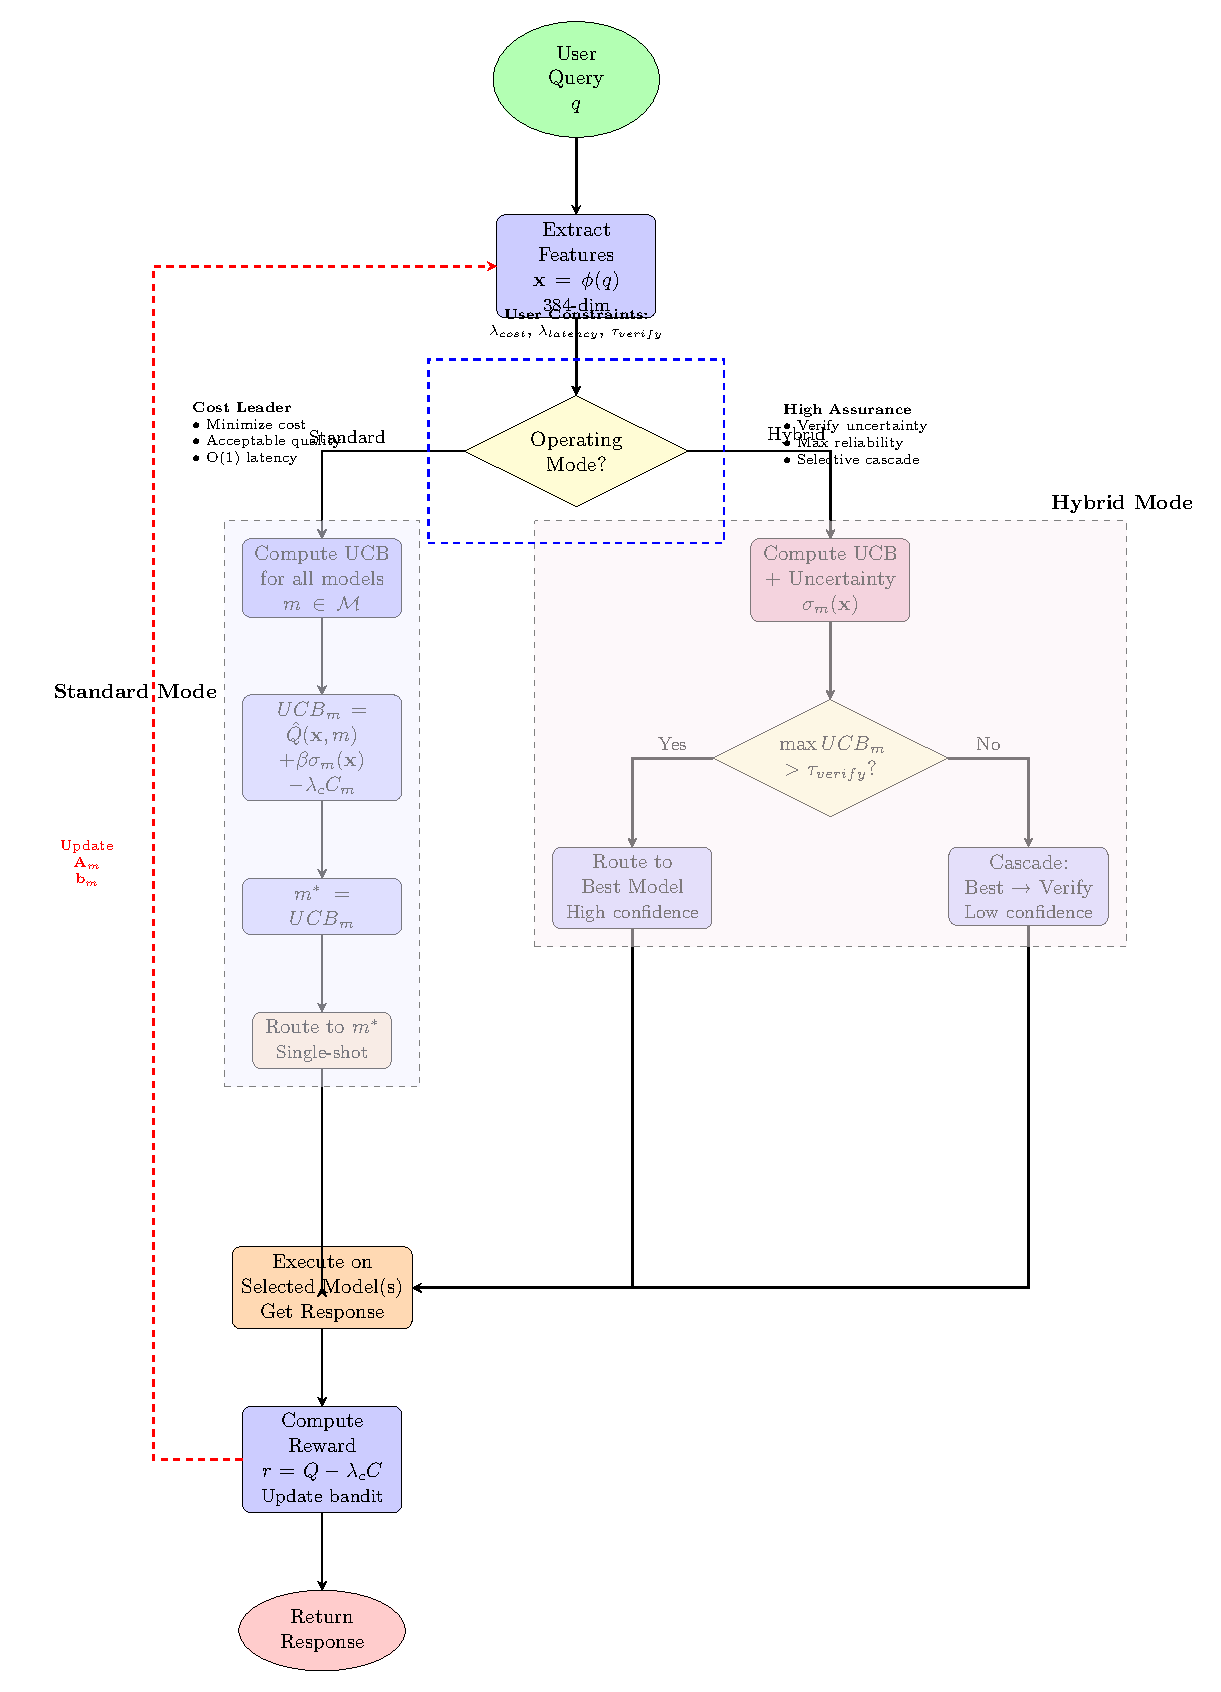
\includegraphics[width=\columnwidth]{figures/decision_tree_diagram.pdf}
    \caption{\textbf{Routing Decision Flow.} Users control system behavior via operating mode and sensitivity parameters. Standard mode (left path) provides single-shot UCB routing optimized for cost leadership, suitable for students and startups. Hybrid mode (right path) performs uncertainty-aware routing, triggering selective verification for low-confidence predictions to ensure high assurance for enterprises. Online feedback continuously updates bandit parameters ($\mathbf{A}_m$, $\mathbf{b}_m$) in both modes, enabling autonomous adaptation to model evolution and distribution drift.}
    \label{fig:routing_logic}
\end{figure}

\begin{table}[t]
\centering
\small
\caption{\textbf{Fixed vs.\ Dynamic Cascade.} Our hybrid enables single-pass routing over a large pool while retaining cascade reliability when needed.}
\label{tab:scaling_comparison}
\begin{tabular}{lcc}
\toprule
\textbf{Property} & \textbf{FrugalGPT} & \textbf{Ours} \\
\midrule
Model Pool & 2--3 & 80+ \\
Sequential Calls & Yes & No (unless verification triggers) \\
Specialist Access & Poor & Excellent \\
Adaptation & None & Online \\
\bottomrule
\end{tabular}
\end{table}

The bandit provides single-pass scoring over 80+ models, unlocking specialists that fixed chains miss; the selective cascade provides a safety net (Table~\ref{tab:scaling_comparison}).
